\subsection{Configure GBTx to use external \itwoc adapter}
\label{sec:hardware-ext-i2c}
This setup is required to program a GBTx board using an external \itwoc adapter.
Follow \autoref{fig:external_i2c} to connect an external \itwoc adapter.

\begin{figure}[!ht]
\centering
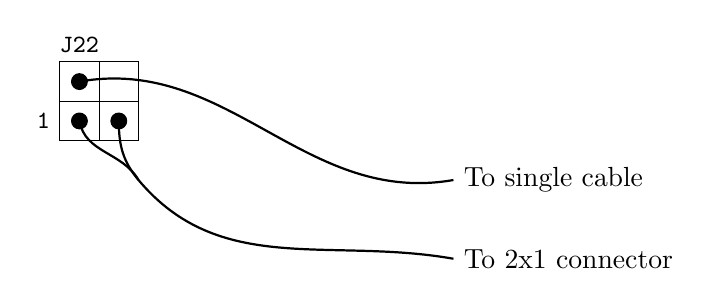
\begin{tikzpicture}
    % Pins
    \draw (0,0) rectangle (0.5,0.5);
    \draw (0.5,0) rectangle (1,0.5);
    \draw (0,-0.5) rectangle (0.5,0);
    \draw (0.5,-0.5) rectangle (1,0);

    % PCB labels
    \coordinate (A) at (0.25,0.5);
    \node at (A) [above] {\small\texttt{J22}};
    \coordinate (B) at (0,-0.25);
    \node at (B) [left] {\small\texttt{1}};

    % Single cable on the I2C
    \draw [black,fill] (0.25,0.25) circle [radius=0.1];
    \draw [thick] (0.25,0.25)
        to [out=10,in=190] (5,-1) node [right]
        {To single cable};

    % 2x1 connector on the I2C
    \draw [black,fill] (0.25,-0.25) circle [radius=0.1];
    \draw [black,fill] (0.75,-0.25) circle [radius=0.1];
    \draw [thick] (0.25,-0.25) to [out=-80,in=120] (1,-1);
    \draw [thick] (0.75,-0.25) to [out=-90,in=130] (1,-1);
    \draw [thick] (1,-1)
        to [out=-50,in=170] (5,-2) node [right]
        {To 2x1 connector};
\end{tikzpicture}
\caption{Schematic for external \itwoc adapter setup.}
\label{fig:external_i2c}
\end{figure}

\begin{leftbar}
    The \itwoc adapter used in our lab is made in-house.
    For the 2x1 connector, make sure the side that has \emph{no} metal contact
    is facing up.
\end{leftbar}
